Dopo aver calcolato le matrici che caratterizzano il sistema semaforico di base, si procede a imporre dei vincoli per evitare che si creino situazioni pericolose o non desiderate. In particolare, si vuole evitare che i seguenti attraversamenti avvengano in contemporanea:

\begin{itemize}
    \item Da Est a Sud, da Ovest a Sud e da Nord a Sud;
    \item Da Ovest a Nord e da Est a Nord;
    \item Da Est a Ovest e da Nord a Ovest;
    \item Da Ovest a Nord e da Est a Ovest;
    \item Da Nord a Sud e da Est a Ovest;
    \item Da Ovest a Nord e da Nord a Sud.
    
\end{itemize}

Qualsiasi altra combinazione in contemporanea è consentita. Le combinazioni appena elencate sono vietate in quanto le prime tre prevedono il passaggio di veicoli provenienti da direzioni diverse e diretti verso la medesima direzione, creando un punto di conflitto in prossimità della direzione di arrivo. Le altre tre combinazioni, invece, sono vietate perchè vedono in contemporanea il passaggio di più veicoli provenienti da direzioni diverse ma che devono attraversare il centro dell'incrocio, generando così un altro punto di conflitto. Per implementare ciò, sono stati imposti i seguenti vincoli:

\begin{itemize}
    \item $M_{2} + M_{14} + M_{26} \leq 1$
    \item $M_{1} + M_{13} + M_{25} \leq 1$
    \item $M_{6} + M_{18} \leq 1$
    \item $M_{5} + M_{17} \leq 1$
    \item $M_{10} + M_{22} \leq 1$
    \item $M_{9} + M_{21} \leq 1$
    \item $M_{6} + M_{22} \leq 1$
    \item $M_{5} + M_{21} \leq 1$
    \item $M_{14} + M_{22} \leq 1$
    \item $M_{13} + M_{21} \leq 1$
    \item $M_{6} + M_{14} \leq 1$
    \item $M_{5} + M_{13} \leq 1$
\end{itemize}

Dopo aver delineato le GMEC, è possibile scriverle in forma matriciale per poi andare a calcolare le posizioni dei supervisori. Otteniamo quindi la matrice descritta nella tabella \ref{tab:w_matrix}:

\begin{table}[ht]
    \centering
    \resizebox{\textwidth}{!}{
        \begin{tabular}{|c|*{28}{c|}}
            \hline
            \rowcolor{lightgray}
            & T0 & T1 & T2 & T3 & T4 & T5 & T6 & T7 & T8 & T9 & T10 & T11 & T12 & T13 & T14 & T15 & T16 & T17 & T18 & T19 & T20 & T21 & T22 & T23 & T24 & T25 & T26 & T27 \\
            \hline
            w1 & 0 & 0 & 1 & 0 & 0 & 0 & 0 & 0 & 0 & 0 & 0 & 0 & 0 & 0 & 1 & 0 & 0 & 0 & 0 & 0 & 0 & 0 & 0 & 0 & 0 & 0 & 1 & 0 \\
            \hline
            w2 & 0 & 1 & 0 & 0 & 0 & 0 & 0 & 0 & 0 & 0 & 0 & 0 & 0 & 1 & 0 & 0 & 0 & 0 & 0 & 0 & 0 & 0 & 0 & 0 & 0 & 1 & 0 & 0 \\
            \hline
            w3 & 0 & 0 & 0 & 0 & 0 & 0 & 1 & 0 & 0 & 0 & 0 & 0 & 0 & 0 & 0 & 0 & 0 & 0 & 1 & 0 & 0 & 0 & 0 & 0 & 0 & 0 & 0 & 0 \\
            \hline
            w4 & 0 & 0 & 0 & 0 & 0 & 1 & 0 & 0 & 0 & 0 & 0 & 0 & 0 & 0 & 0 & 0 & 0 & 1 & 0 & 0 & 0 & 0 & 0 & 0 & 0 & 0 & 0 & 0 \\
            \hline
            w5 & 0 & 0 & 0 & 0 & 0 & 0 & 0 & 0 & 0 & 0 & 1 & 0 & 0 & 0 & 0 & 0 & 0 & 0 & 0 & 0 & 0 & 0 & 1 & 0 & 0 & 0 & 0 & 0 \\
            \hline
            w6 & 0 & 0 & 0 & 0 & 0 & 0 & 0 & 0 & 0 & 1 & 0 & 0 & 0 & 0 & 0 & 0 & 0 & 0 & 0 & 0 & 0 & 1 & 0 & 0 & 0 & 0 & 0 & 0 \\
            \hline
            w7 & 0 & 0 & 0 & 0 & 0 & 0 & 1 & 0 & 0 & 0 & 0 & 0 & 0 & 0 & 0 & 0 & 0 & 0 & 0 & 0 & 0 & 0 & 1 & 0 & 0 & 0 & 0 & 0 \\
            \hline
            w8 & 0 & 0 & 0 & 0 & 0 & 1 & 0 & 0 & 0 & 0 & 0 & 0 & 0 & 0 & 0 & 0 & 0 & 0 & 0 & 0 & 0 & 1 & 0 & 0 & 0 & 0 & 0 & 0 \\
            \hline
            w9 & 0 & 0 & 0 & 0 & 0 & 0 & 0 & 0 & 0 & 0 & 0 & 0 & 0 & 0 & 1 & 0 & 0 & 0 & 0 & 0 & 0 & 0 & 1 & 0 & 0 & 0 & 0 & 0 \\
            \hline
            w10 & 0 & 0 & 0 & 0 & 0 & 0 & 0 & 0 & 0 & 0 & 0 & 0 & 0 & 1 & 0 & 0 & 0 & 0 & 0 & 0 & 0 & 1 & 0 & 0 & 0 & 0 & 0 & 0 \\
            \hline
            w11 & 0 & 0 & 0 & 0 & 0 & 0 & 1 & 0 & 0 & 0 & 0 & 0 & 0 & 0 & 1 & 0 & 0 & 0 & 0 & 0 & 0 & 0 & 0 & 0 & 0 & 0 & 0 & 0 \\
            \hline
            w12 & 0 & 0 & 0 & 0 & 0 & 1 & 0 & 0 & 0 & 0 & 0 & 0 & 0 & 1 & 0 & 0 & 0 & 0 & 0 & 0 & 0 & 0 & 0 & 0 & 0 & 0 & 0 & 0 \\
            \hline
        \end{tabular}
    }
    \caption{Matrice W}
    \label{tab:w_matrix}
\end{table}

Utilizzando quindi la formula \ref{eq:gmec_vect}, possiamo quindi calcolare le righe da aggiungere alla matrice di incidenza per indicare i nuovi posti monitor:

\begin{table}[ht]
    \centering
    \resizebox{\textwidth}{!}{
        \begin{tabular}{|c|*{28}{c|}}
            \hline
            \rowcolor{lightgray}
            & T0 & T1 & T2 & T3 & T4 & T5 & T6 & T7 & T8 & T9 & T10 & T11 & T12 & T13 & T14 & T15 & T16 & T17 & T18 & T19 & T20 & T21 & T22 & T23 & T24 & T25 & T26 & T27 \\
            \hline
            P28 & 1 & -1 & 1 & -1 & 0 & 0 & 0 & 0 & 0 & 0 & 0 & 0 & 1 & -1 & 1 & -1 & 0 & 0 & 0 & 0 & 0 & 0 & 0 & 0 & 1 & -1 & 1 & -1 \\
            \hline
            P29 & -1 & 1 & 0 & 0 & 0 & 0 & 0 & 0 & 0 & 0 & 0 & 0 & -1 & 1 & 0 & 0 & 0 & 0 & 0 & 0 & 0 & 0 & 0 & 0 & -1 & 1 & 0 & 0 \\
            \hline
            P30 & 0 & 0 & 0 & 0 & 1 & -1 & 1 & -1 & 0 & 0 & 0 & 0 & 0 & 0 & 0 & 0 & 1 & -1 & 1 & -1 & 0 & 0 & 0 & 0 & 0 & 0 & 0 & 0 \\
            \hline
            P31 & 0 & 0 & 0 & 0 & -1 & 1 & 0 & 0 & 0 & 0 & 0 & 0 & 0 & 0 & 0 & 0 & -1 & 1 & 0 & 0 & 0 & 0 & 0 & 0 & 0 & 0 & 0 & 0 \\
            \hline
            P32 & 0 & 0 & 0 & 0 & 0 & 0 & 0 & 0 & 1 & -1 & 1 & -1 & 0 & 0 & 0 & 0 & 0 & 0 & 0 & 0 & 1 & -1 & 1 & -1 & 0 & 0 & 0 & 0 \\
            \hline
            P33 & 0 & 0 & 0 & 0 & 0 & 0 & 0 & 0 & -1 & 1 & 0 & 0 & 0 & 0 & 0 & 0 & 0 & 0 & 0 & 0 & -1 & 1 & 0 & 0 & 0 & 0 & 0 & 0 \\
            \hline
            P34 & 0 & 0 & 0 & 0 & 1 & -1 & 1 & -1 & 0 & 0 & 0 & 0 & 0 & 0 & 0 & 0 & 0 & 0 & 0 & 0 & 1 & -1 & 1 & -1 & 0 & 0 & 0 & 0 \\
            \hline
            P35 & 0 & 0 & 0 & 0 & -1 & 1 & 0 & 0 & 0 & 0 & 0 & 0 & 0 & 0 & 0 & 0 & 0 & 0 & 0 & 0 & -1 & 1 & 0 & 0 & 0 & 0 & 0 & 0 \\
            \hline
            P36 & 0 & 0 & 0 & 0 & 0 & 0 & 0 & 0 & 0 & 0 & 0 & 0 & 1 & -1 & 1 & -1 & 0 & 0 & 0 & 0 & 1 & -1 & 1 & -1 & 0 & 0 & 0 & 0 \\
            \hline
            P37 & 0 & 0 & 0 & 0 & 0 & 0 & 0 & 0 & 0 & 0 & 0 & 0 & -1 & 1 & 0 & 0 & 0 & 0 & 0 & 0 & -1 & 1 & 0 & 0 & 0 & 0 & 0 & 0 \\
            \hline
            P38 & 0 & 0 & 0 & 0 & 1 & -1 & 1 & -1 & 0 & 0 & 0 & 0 & 1 & -1 & 1 & -1 & 0 & 0 & 0 & 0 & 0 & 0 & 0 & 0 & 0 & 0 & 0 & 0 \\
            \hline
            P39 & 0 & 0 & 0 & 0 & -1 & 1 & 0 & 0 & 0 & 0 & 0 & 0 & -1 & 1 & 0 & 0 & 0 & 0 & 0 & 0 & 0 & 0 & 0 & 0 & 0 & 0 & 0 & 0 \\
            \hline
        \end{tabular}
    }
    \caption{Matrice di incidenza con i posti monitor}
    \label{tab:inc_matrix}
\end{table}

Utilizzando poi la formula \ref{eq:gmec_init} è poi possibile calcolare la marcatura iniziale di tutti i posti monitor. Nel caso in esame, la marcatura di tutti i postimonitor è pari a 1.

\begin{figure}[H]
    \centering
    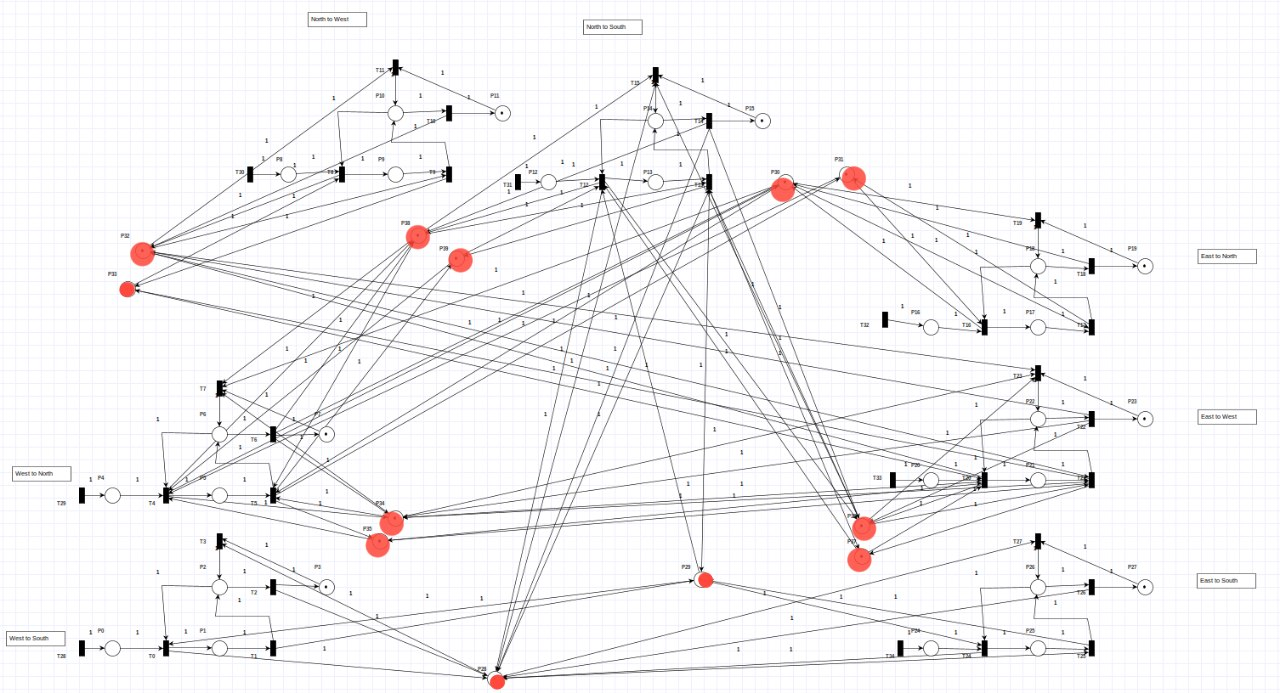
\includegraphics[width=1.0\textwidth]{figure/project_screenshots/sem_fin_controlli_evidenziati.jpg}
    \caption{Rete di Petri con i posti monitor evidenziati}
    \label{fig:petri_supervisori}
\end{figure}